% 2.2.PrepareLibrary.tex
%	Last update: 2019/12/04 F.Kanehori
%newpage
\subsection{準備}
\label{subsec:PrepareLibrary}

\noindent
ダウンロードが済んだら\SprTop{/core/src}に移動してください。

\noindent
まず、配布されたファイル\CMakeLists{.Lib.dist}を
\CMakeLists{}という名前でコピーします
(誤コミットを防止するためにもリネームではなくコピーしてください)。

\medskip
\ifLwarp
	\begin{figure}[h]
	    \begin{center}
	    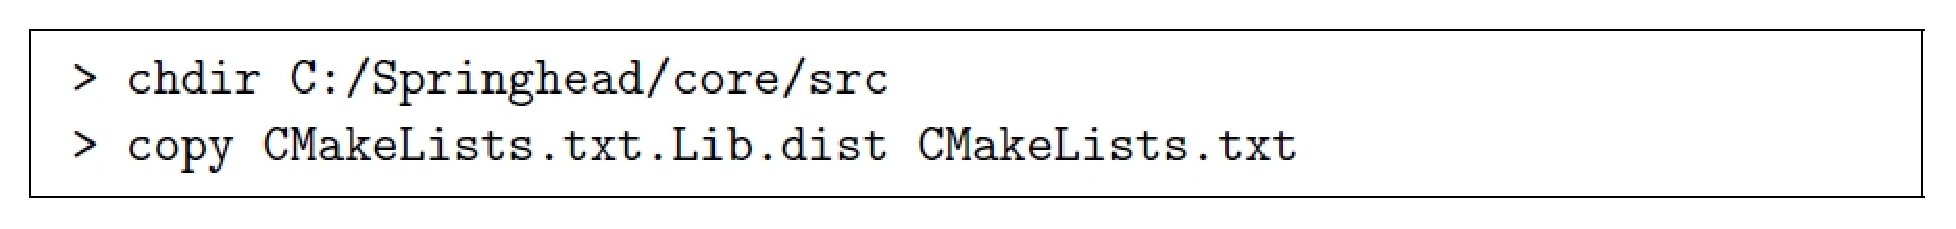
\includegraphics[width=\textwidth]{fig/command-2-2-a.eps}
	    \end{center}
	    \label{fig:DownloadTree}
	\end{figure}
\else
\begin{narrow}[15pt]
	\CmndBox{%
		> chdir C:/Springhead/core/src\\
		> copy CMakeLists.txt.Lib.dist CMakeLists.txt
	}
\end{narrow}
\fi

\medskip
\noindent
自前でインストールしているパッケージ
(\tt{boost}, \tt{glew}, \tt{freeglut}, \tt{glui})を使用する場合
およびライブラリファイルとヘッダファイルのインストール先を指定する場合には、
さらに、
配布されたファイル\CMakeConf{.dist}を\CMakeConf{}という名前でコピーして
必要な編集をします。
編集の方法については\CMakeConf{}に記述されています
(``\tt{\#set(variable \it{value})}''から``\tt{\#}''を削除し、
``\it{value}''を適切に設定し直す)。

\def\cite#1{\hspace{10pt}\footnotesize{#1}}
\def\somewhere{"C:/\it{somewhere}/\it{appropreate}"}
\medskip
\ifLwarp
	\begin{figure}[h]
	    \begin{center}
	    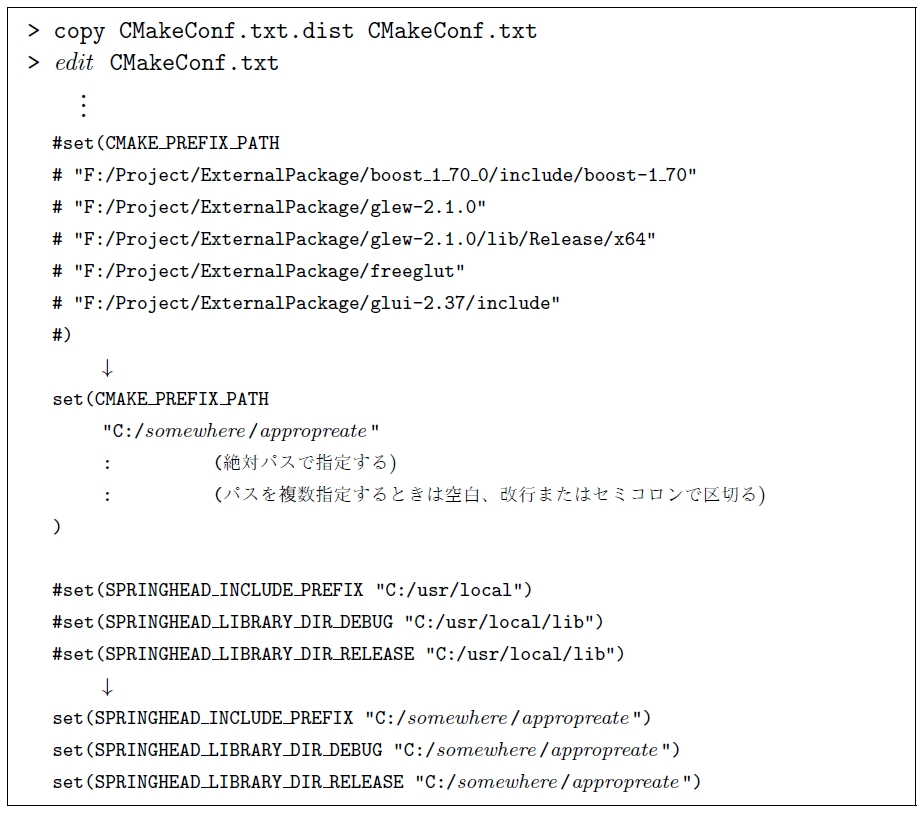
\includegraphics[width=\textwidth]{fig/command-2-2-b.eps}
	    \end{center}
	    \label{fig:DownloadTree}
	\end{figure}
\else
\begin{narrow}[15pt]
	\CmndBox{%
		> copy CMakeConf.txt.dist CMakeConf.txt\\
		> \it{edit} CMakeConf.txt\\
		\hspace{20pt}$\vdots$\\
	\cite{\#set(CMAKE\_PREFIX\_PATH}\\
	\cite{\# "F:/Project/ExternalPackage/boost\_1\_70\_0/include/boost-1\_70"}\\
	\cite{\# "F:/Project/ExternalPackage/glew-2.1.0"}\\
	\cite{\# "F:/Project/ExternalPackage/glew-2.1.0/lib/Release/x64"}\\
	\cite{\# "F:/Project/ExternalPackage/freeglut"}\\
	\cite{\# "F:/Project/ExternalPackage/glui-2.37/include"}\\
	\cite{\#)}\\
	\cite{\hspace{20pt}$\downarrow$}\\
	\cite{set(CMAKE\_PREFIX\_PATH}\\
	\cite{\hbox to 20pt{}\somewhere}\\
	\cite{\hspace{20pt}:\hspace{40pt}{(\rm{絶対パスで指定する)}}}\\
	\cite{\hspace{20pt}:\hspace{40pt}%
		{(\rm{パスを複数指定するときは空白、改行またはセミコロンで区切る)}}}\\
	\cite{)}\\
	\cite{}\\
	\cite{\#set(SPRINGHEAD\_INCLUDE\_PREFIX       "C:/usr/local")}\\
	\cite{\#set(SPRINGHEAD\_LIBRARY\_DIR\_DEBUG   "C:/usr/local/lib")}\\
	\cite{\#set(SPRINGHEAD\_LIBRARY\_DIR\_RELEASE "C:/usr/local/lib")}\\
	\cite{\hspace{20pt}$\downarrow$}\\
	\cite{set(SPRINGHEAD\_INCLUDE\_PREFIX       \somewhere)}\\
	\cite{set(SPRINGHEAD\_LIBRARY\_DIR\_DEBUG   \somewhere)}\\
	\cite{set(SPRINGHEAD\_LIBRARY\_DIR\_RELEASE \somewhere)}
	}
\end{narrow}
\fi

\medskip
\noindent
コンパイル及びリンクのオプションはファイル\CMakeOpts{.dist}に設定されています。
これらのオプションを変更するときは、配布されたファイル\CMakeOpts{.dist}を
\CMakeOpts{}という名前でコピーして必要な編集をします。

\medskip
\noindent
以上で準備作業は終了です。

% end: 2.2.PrepareLibrary.tex
